\documentclass[a4paper, 12pt]{article}
\usepackage{graphicx} % Required for inserting images
\usepackage{fullpage}
\usepackage{amsmath}
\usepackage{xcolor}
\usepackage{float}
\usepackage{geometry}
\usepackage{biblatex}
\geometry{margin=1in}
\usepackage{enumitem}
\usepackage{hyperref}
\usepackage{parskip}
\title{Chemistry Honors Study Guide}
\author{Test 2 S1}
\date{Test date: October 18, 2024}

\begin{document}

\maketitle

\begin{center}
    (All links are clickable!)
\end{center}

\section{Forming Ionic Compounds}

\subsection*{Definitions}
\begin{itemize}[leftmargin=*,nosep]
\item \textbf{\emph{ion:}} Charged particle.
\item \textbf{\emph{cation:}} Positively charged particle. All cations are metals.
\item \textbf{\emph{anion:}} Negatively charged particle. All anions are either nonmetals or metalloids.
\item \textbf{\emph{ionic compound:}} Created from electrostatic attraction between cations and anions.
\item \textbf{\emph{salt:}} Another name for an ionic compound.
\end{itemize}

\subsection*{Ionic Bonding}
Atoms form bonds to fill their valence shells. Depending on what is easier for an atom of each element (getting rid of/gaining electrons), they will have a positive or negative charge.
 
Once bonded, the charges on each ion must cancel out. Like fraction addition, we change the charges to their least common multiple (if they are not already equal).
 
Example: \textcolor{blue}{2K$^{\text{1+}}$ + O$^{\text{2-}}$ $\xrightarrow{}$ K$_2$O} \textbf{cation first!}
 
After the bonding occurs, the charge on the resulting particle is neutral.

\section{Naming Ionic Compounds}
\subsection*{Definitions}
\begin{itemize}[leftmargin=*,nosep]
    \item \textbf{\emph{Type I cation:}} Includes groups 1, 2, 13, Ag$+$, Zn$^{\text{2+}}$. Can only have a single charge state.
    \item \textbf{\emph{Type II cation:}} Transition metals (not Ag or Zn), Pb, Sn. Can have multiple charge states.
\end{itemize}

\subsection*{Naming Compounds with Type I Cations (Monatomic Anions)}
\fbox {\textcolor{blue}{\textbf{name of cation + anion ending in -ide}}}
 
Example: \textcolor{blue}{Al$_2$S$_3$: Aluminum sulfide}  
Note that the number of atoms present does not influence the naming.

\subsection*{Naming Compounds with Type II Cations (Monatomic Anions)}
\fbox {\textcolor{blue}{\textbf{cation + charge on cation + anion ending in -ide}}}
 
Example: \textcolor{blue}{Fe$_2$O$_3$: iron (III) oxide}
 
In this example, the number of iron atoms does not matter; the number in parentheses is always the charge.

\subsection*{Naming Compounds with Polyatomic Anions}
\begin{itemize}[leftmargin=*,nosep]
    \item NO$_3$$^-$: \textbf{nitrate}
    \item ClO$_3$$^-$: \textbf{chlorate}
    \item CO$_3$$^{\text{2-}}$: \textbf{carbonate}
    \item SO$_4$$^{\text{2-}}$: \textbf{sulfate}
    \item PO$_4$$^{\text{3-}}$: \textbf{phosphate}
\end{itemize}
|||||||||||||||||||||||||||||||||||

\noindent \textbf{\underline{N}\textcolor{red}{i}ck the \underline{C}\textcolor{red}{a}m\textcolor{red}{e}l ate \underline{Cl}\textcolor{red}{a}m \underline{S}\textcolor{red}{u}pp\textcolor{red}{e}r in \underline{P}h\textcolor{red}{oe}n\textcolor{red}{i}x}
 
\textbf{Number of consonants:} Number of oxygen atoms
\\
\textbf{\textcolor{red}{Number of vowels:}} Number of negative charges

\noindent |||||||||||||||||||||||||||||||||||
\begin{table}[ht]
    \centering
    \begin{tabular}{c|c|c|c}
         \textbf{Relative \# of Oxygen } & \textbf{Prefix/suffix} & \textbf{Equation} & \textbf{Name} \\\hline
        +1 & per...ate & ClO$_4$$^-$ & perchlorate \\
        -1 & -ite & ClO$_2$$^-$ & chlorite \\
        0 & -ate & ClO$_3$$^-$ & chlorate \\
        -2 & hypo...ite & ClO$^-$ & hypochlorite
    \end{tabular}
    \label{tab:my_label}
\end{table}

\noindent Example: \textcolor{blue}{PO$_5$$^{\text{3-}}$: perphosphate}; \textcolor{blue}{Na$_3$PO$_5$: sodium perphosphate}
 
(Note that the charge does not change with the number of oxygen atoms, but when the polyatomic anion bonds with a cation, the resulting compound becomes neutral.)

\section{Covalent Compounds}

\subsection*{Definitions}
\begin{itemize}[leftmargin=*,nosep]
    \item \textbf{\emph{covalent compound:}} A compound bonded covalently (sharing valence electrons).
\end{itemize}

\subsection*{Naming Binary Covalent Compounds (two elements)}
\fbox {\textbf{\textcolor{blue}{if $>$ 1, number prefix + first element + number prefix + second element + -ide}}} %fix this part
 
Example: \textcolor{blue}{N$_2$O$_3$: \textbf{di}nitrogen \textbf{tri}oxide}

\subsubsection*{Prefixes:}
\begin{enumerate}[leftmargin=*,nosep]
    \item \textbf{mono}-
    \item \textbf{di}-
    \item \textbf{tri}-
    \item \textbf{tetra}-
    \item \textbf{penta}-
    \item \textbf{hexa}-
    \item \textbf{hepta}-
    \item \textbf{octa}-
\end{enumerate}

\section{Identification and Diagrams}

\subsection*{Identifying Ionic vs Covalent Compounds}

\subsubsection*{Ionic compounds...}
\begin{itemize}[leftmargin=*,nosep]
    \item start with a \textbf{metal} or with \textbf{NH$_4$$^+$} (ammonium).
    \item form from the electrostatic attraction of \textbf{metals with nonmetals/metalloids}.
\end{itemize}

\subsubsection*{Covalent compounds...}
\begin{itemize}[leftmargin=*,nosep]
    \item are formed between \textbf{metals or metalloids}.
    \item involve the \textbf{sharing of electrons}.
\end{itemize}

\subsection*{Lattice Diagrams}

\subsubsection*{Essential aspects of lattice diagrams:}
\begin{itemize}[leftmargin=*,nosep]
    \item separated charges (- not touching +)
    \item atomic ratio
    \item atomic symbol
    \item at least 2 repetitions
\end{itemize}

\subsubsection*{Identifying Covalent Lattice Diagrams}
\textbf{Molecular:} distinct molecules, not interconnected (such as H$_2$O)
\\
\textbf{Network:} interconnected network of atoms (such as C (diamond))

\subsubsection*{Ionic Lattice Diagrams\footnote{https://www.elevise.co.uk/gac2c.html}}

Example: \textcolor{blue}{NaCl (sodium chloride/table salt)}

\begin{figure}[ht]
    \centering
    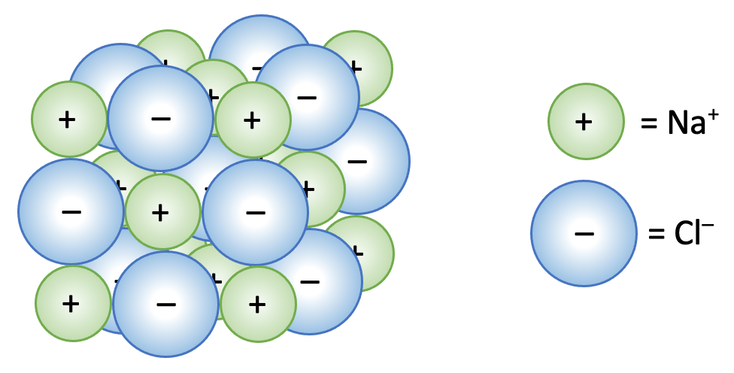
\includegraphics[width=0.5\linewidth]{lattice.png} 
    \label{fig:1}
\end{figure} 

\subsubsection*{Metallic Lattice Diagrams\footnote{https://www.savemyexams.com/ap/chemistry/college-board/22/revision-notes/unit-2-molecular-and-ionic-compound-structure-and-properties/2-4-structure-of-metals-and-alloys/representing-metallic-bonding/}}

\begin{figure}[ht]
    \centering
    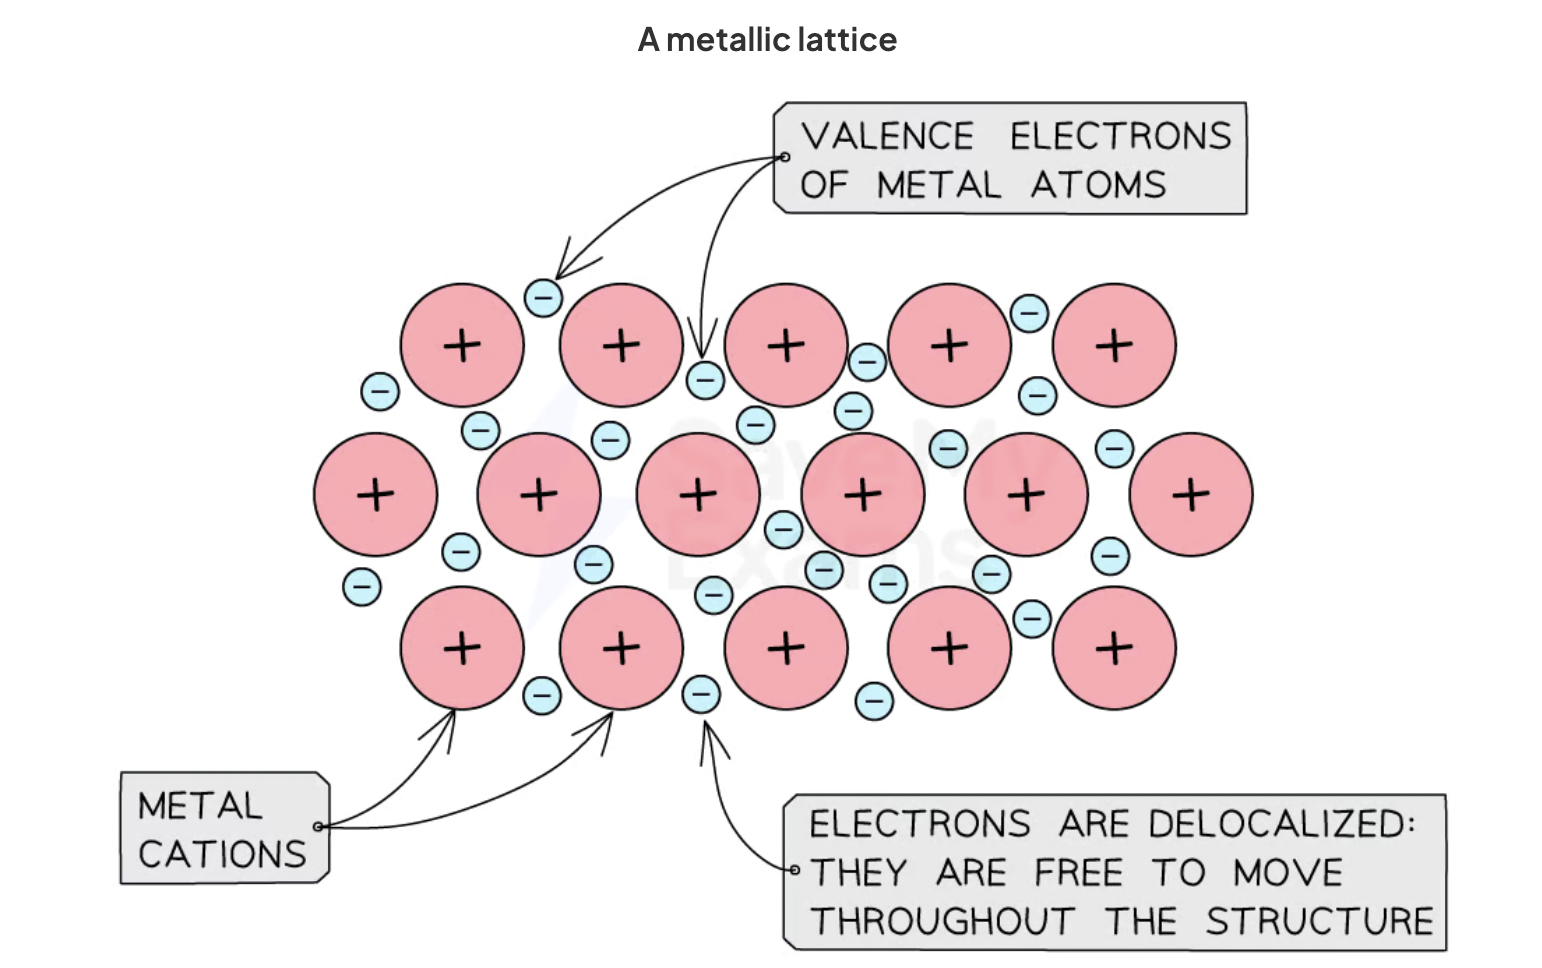
\includegraphics[width=0.5\linewidth]{metalliclattice.png}
    \label{fig:1.3?}
\end{figure}
\noindent (This is the diagram for all metallic bonding. The number of atoms, electrons, and arrow directions do not matter as long as the picture shows a cluster of atoms with moving electrons.)

\subsection*{Lewis Dot Structures}

\subsubsection*{Atomic LDS\footnote{https://americanboard.org/Subjects/general-science/bonding-and-atomic-structure/}
}

\begin{figure}[htbp] 
    \centering
    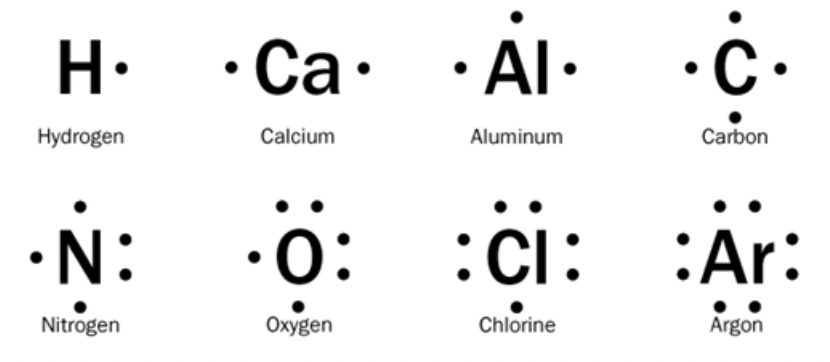
\includegraphics[width=0.5\linewidth]{atomiclds.png}
    \label{fig:2}
\end{figure} 
\noindent As shown above, the number of valence electrons increases as you go across the periodic table, so the number of dots increase. (Placement is intentional -- when drawing the atomic structures, electrons are separated, but in ionic/covalent structures, electrons are drawn in pairs.)

\subsubsection*{Ionic LDS\footnote{https://scienceready.com.au/pages/lewis-dot-diagram}}
\begin{itemize}[leftmargin=*,nosep]
    \item The \textbf{cation} always has an \textbf{empty valence shell} (no dots).
    \item The \textbf{anion} always has a \textbf{filled valence shell} with \textbf{brackets} around the atom.
    \item \textbf{Charges should be indicated} in the top right of each atom.
    \item Charges are \textbf{properly separated.}
\end{itemize}



\begin{figure}[ht]
    \centering
    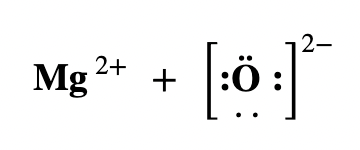
\includegraphics[width=0.5\linewidth]{ioniclds.png}
    \label{fig:2.5}
\end{figure}

\noindent Example: \textcolor{blue}{MgO (magnesium oxide)}

\subsubsection*{Covalent LDS\footnote{https://byjus.com/chemistry/carbon-disulfide/}}
\begin{enumerate}[leftmargin=*,nosep]
    \item Determine the \textbf{number of valence electrons.}
    \item Determine the \textbf{central atom} if there are more than 2 atoms. \textbf{The central atom (with the exception of hydrogen) should be the one with the lowest electronegativity.}
    \item \textbf{Draw the LDS} so that \textbf{each atom (note exceptions below) has a full valence shell.}
    \item Replace shared electrons with lines. \textbf{(2 electrons = 1 bond = 1 line).}
\end{enumerate}


\begin{figure}[ht]
    \centering
    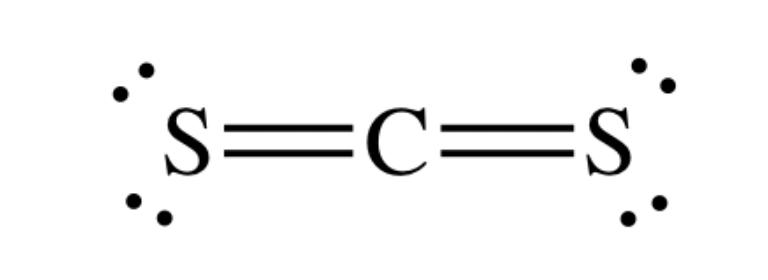
\includegraphics[width=0.3\linewidth]{covalentlds.png}
    \label{fig:3}
\end{figure}

\noindent Example: \textcolor{blue}{CS$_2$ (carbon disulfide)}

\subsubsection*{Exceptions\footnote{https://www.fishersci.ca/shop/products/phosphorus-v-chloride-98-thermo-scientific/p-3257053}}
\begin{itemize}[leftmargin=*,nosep]
    \item \textbf{Hydrogen} forms a \textbf{full duet} (2 valence electrons).
    \item \textbf{Boron} forms a \textbf{full sestet} (6 valence electrons).
    \item Elements in the \textbf{third period or below} may have an \textbf{expanded octet} (more than 8 electrons in their valence shell).
\end{itemize}


\begin{figure}[ht]
    \centering
    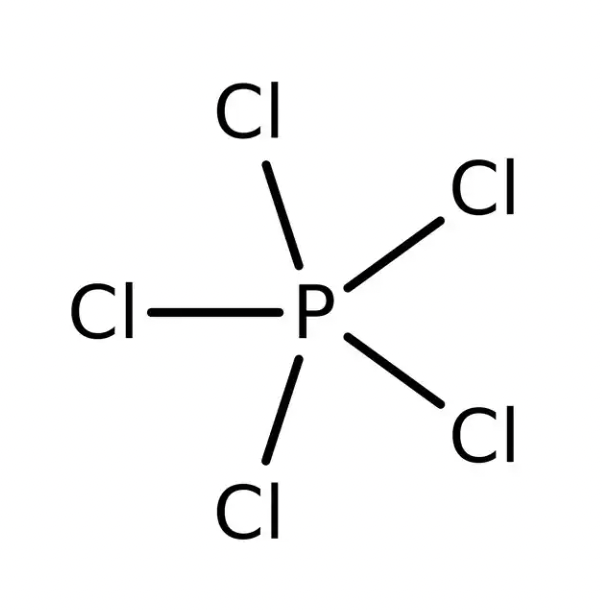
\includegraphics[width=0.2\linewidth]{exceptionlds.png}
    \label{fig:4}
\end{figure}

\noindent Example: \textcolor{blue}{PCl$_5$ (phosphorus pentachloride)}

\subsubsection*{Polyatomic Ions}
Polyatomic ions are \textit{covalent structures within an ionic structure.} Draw the Lewis dot structure of a polyatomic ion as a covalent compound, treating it as a single unit, then add the element it bonds ionically with to the diagram. As usual, include brackets when necessary.
 
When making LDS with polyatomic ions that have expanded octets, the \textbf{formal charge on the central atom must equal 0.} The formula to find formal charge of an atom is as follows: 
 $$ \text{formal charge = \# of valence electrons} - \text{\# of lone pair electrons} - \text{\# of bonds} $$

\noindent Note that the number of lone pair electrons refers to the number of individual electrons, not the number of lone pairs. (Formal charge does not need to be indicated unless the problem states otherwise.)

\begin{figure}[ht]
    \centering
    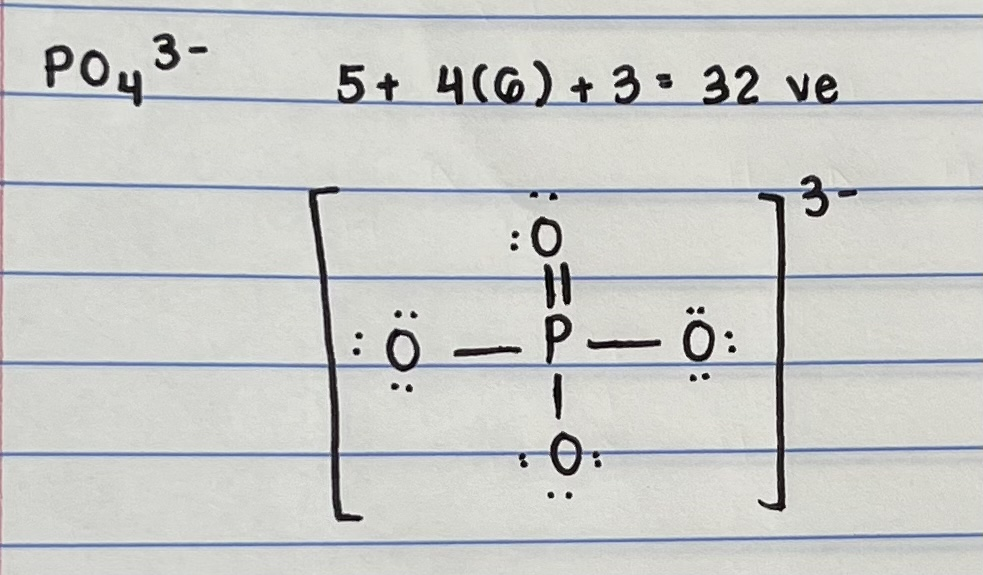
\includegraphics[width=0.5\linewidth]{expandedlds.jpeg}
    \label{fig:enter-label}
\end{figure}
\noindent Example: \textcolor{blue}{PO$_4$$^3-$ (phosphate)}

\section{Periodic Table Trends}

\subsection*{Definitions}
\begin{itemize}[leftmargin=*, nosep]
    \item \textbf{\textit{effective nuclear charge:}} The force felt by an electron from the nucleus.
    \item \textbf{\textit{electronegativity:}} The tendency of an atom to attract electrons.
    \item \textbf{\textit{ionization energy:}} The energy it takes to remove an electron from an atom.
    \item \textbf{\textit{atomic radius:}} The size of the atom, or, more precisely, the distance from an atom's nucleus to its outermost orbital.
\end{itemize}

\subsection*{Coulomb's Law}

$$F = k\frac{q_1q_2}{r^2}$$

where:
\begin{itemize}[nosep]
    \item $F$ = force felt by electron
    \item $k$ = Coulomb's constant (not important for this test)
    \item $q_1$ = charge on valence electron
    \item $q_2$ = charge on nucleus
    \item $r$ = distance (nucleus to electron)
\end{itemize}

\subsection*{Electronegativity and Ionization Energy}
Electronegativity and ionization energy \textbf{increase} as you go \textbf{higher} and to the \textbf{right} in the periodic table.
 
Electronegativity increases near the top of the periodic table because the distance from the potential electron and the nucleus is smaller (as described by Coulomb's Law above.) Near the right, electronegativity increases because the atoms grow increasingly close to filling their valence shells, needing to attract extra electrons.
 
Ionization energy increases near the top because it is harder to remove an electron close to the nucleus (again, as described by Coulomb's Law). Near the right, ionization energy increases because it becomes increasingly difficult to remove electrons from atoms that are close to filling their valence shells.

\subsection*{Atomic Radii}
The atomic radius \textbf{increases} as you go \textbf{lower} and to the \textbf{left} in the periodic table. This is because as the number of protons increases (as you go to the right), it will pull the electrons closer, resulting in a smaller atomic radius, and as the number of orbitals increases (as you go lower), the atomic radius increases likewise.


\end{document}

